\section{Các giải pháp học sâu trong bài toán nhận diện khuôn mặt}

%Tổng quan về các giải pháp học sâu, các bài review,...
Năm 2014 đánh dấu bước ngoặt quan trọng khi các phương pháp học sâu đạt độ chính xác ngang mức con người trong bài toán nhận diện khuôn mặt, qua đó thu hút mạnh mẽ sự quan tâm của cộng đồng nghiên cứu và mở ra hướng tiếp cận mới cho lĩnh vực này. Trước đó, nhận diện khuôn mặt đã được nghiên cứu trong nhiều thập kỷ với các hướng tiếp cận chủ yếu như phương pháp toàn diện, hình học và kết cấu cục bộ; tuy nhiên, hiệu năng của các phương pháp này trong điều kiện không kiểm soát vẫn bị giới hạn, điển hình chỉ đạt khoảng 95\% trên tập dữ liệu LFW\cite{2_electronics9081188,20_WANG2021215}. Sự xuất hiện của học sâu đã tạo ra bước nhảy vọt về hiệu năng: chỉ trong vòng một thập kỷ, các mô hình đã đạt độ chính xác lên tới 99.8\% trên LFW, nhờ khả năng tự động học và biểu diễn các đặc trưng phức tạp ở mức độ ngữ nghĩa cao, bao gồm cả đặc trưng khuôn mặt và điều kiện ảnh (ánh sáng, góc nhìn)\cite{21_otoole_2021_face}. Với ưu thế vượt trội này, học sâu nhanh chóng trở thành hướng tiếp cận chủ đạo, thúc đẩy nhiều nghiên cứu tổng ( \cite{2_electronics9081188,20_WANG2021215,30_9145558,sota_5979728,sota_GUO2019102805} ) quan nhằm phân loại, đánh giá mô hình, cũng như phân tích các kỹ thuật xử lý ảnh và những vấn đề liên quan. Chi tiết nội dung các bài tổng hợp được trình bày dưới đây:

Guodong Guo và Na Zhang (2019) \cite{sota_GUO2019102805} đã thực hiện một khảo sát toàn diện, hệ thống hóa 330 công trình nghiên cứu liên quan đến nhận diện khuôn mặt trong giai đoạn 2011-2018. Nghiên cứu này phân tích và so sánh nhiều kiến trúc mạng khác nhau, bao gồm CNN truyền thống, autoencoder, Restricted Boltzmann Machine (RBM), Deep Belief Networks (DBNs), Deep Boltzmann Machines (DBMs), mạng đối nghịch tạo sinh (GAN) và các kiến trúc lai. Bên cạnh đó, các tác giả cũng tổng hợp và đánh giá các phương pháp xử lý những thách thức đặc thù của bài toán như biến đổi tư thế (cross-pose), độ tuổi (cross-age) và các yếu tố biến thiên khác. Ngoài ra, nghiên cứu còn chỉ ra rằng vẫn còn nhiều vấn đề chưa được giải quyết triệt để. Trong số đó, việc thiết kế các kiến trúc học sâu hiệu quả hơn, đồng thời tối ưu hóa mô hình về cả độ chính xác và chi phí tính toán, vẫn là một hướng nghiên cứu tiềm năng và cần thiết trong lĩnh vực này.

Mei Wang và Weihong Deng (2021) \cite{20_WANG2021215} đã thực hiện khảo sát toàn diện về các tiến bộ gần đây trong hệ thống nhận diện khuôn mặt dựa trên học sâu. Nghiên cứu bao quát toàn bộ pipeline, từ tiền xử lý ảnh , kiến trúc mạng, hàm mất mát, phương pháp so khớp/nhận diện, cho đến các bộ dữ liệu phổ biến và các kịch bản ứng dụng cụ thể. Đặc biệt, các hàm mất mát được phân loại thành ba nhóm chính nhằm phục vụ việc phân tích, đánh giá và so sánh một cách hệ thống. Kết quả khảo sát cho thấy, cùng với sự gia tăng ứng dụng trong thực tế và thương mại, nhiều giả định lý tưởng trong môi trường nghiên cứu không còn được đảm bảo. Điều này dẫn đến hàng loạt thách thức mới, bao gồm các vấn đề về an ninh và bảo mật, khả năng giải thích của mô hình (interpretability), bài toán đánh đổi giữa hiệu năng và độ chính xác, cũng như nhu cầu phát triển các mô hình nhận diện lai nhằm đáp ứng các yêu cầu ứng dụng đa dạng.

Nemavhola et al. (2025) \cite{sota_5979728} đã thực hiện khảo sát 266 công trình nghiên cứu trong giai đoạn 2015–2023, tập trung vào các mô hình nhận diện khuôn mặt dựa trên CNN. Nghiên cứu tiến hành hệ thống hóa và phân loại các công trình theo nhiều tiêu chí, bao gồm quốc gia, năm công bố, lĩnh vực ứng dụng, phương pháp học (có giám sát/không giám sát) và tập dữ liệu huấn luyện. Kết quả cho thấy phần lớn các nghiên cứu sử dụng ảnh tĩnh và các bộ dữ liệu đã được làm sạch (clean dataset) để huấn luyện, chủ yếu với các kiến trúc CNN truyền thống. Cách tiếp cận này dẫn đến xu hướng mô hình đạt hiệu năng cao trong môi trường kiểm soát nhưng suy giảm đáng kể khi triển khai trong điều kiện thực tế. Bên cạnh đó, chỉ khoảng 6\% số công trình tập trung vào các hệ thống nhận diện thời gian thực, cho thấy đây vẫn là một hướng nghiên cứu còn hạn chế và cần được quan tâm nhiều hơn trong tương lai.

\begin{figure}[ht]
  \centering
  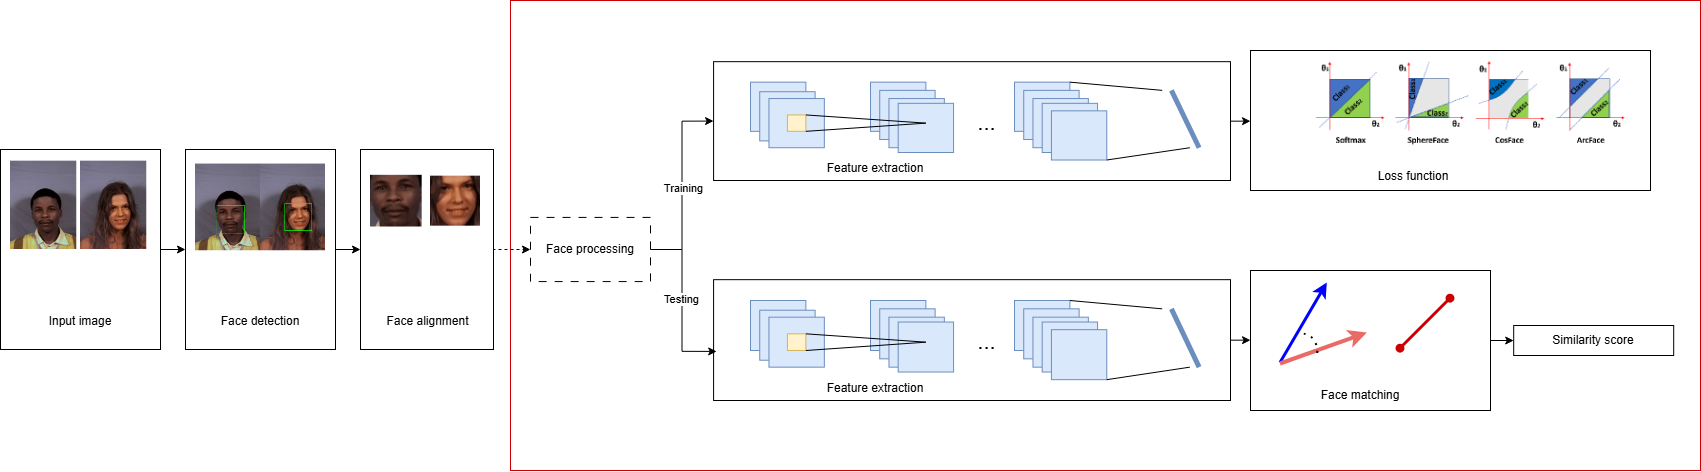
\includegraphics[width=\linewidth]{images/DataPipeline.drawio (1).png}
  \caption[Các bước chính của bài toán xác minh khuôn mặt]{Các bước chính của bài toán xác minh khuôn mặt (Nguồn:  \cite{4_Deng_2019_CVPR,20_WANG2021215})}
  \label{fig:data-pipeline}
\end{figure}
Bài toán xác minh khuôn mặt (face verification) có thể được phân tách thành ba giai đoạn chính: (i) phát hiện và căn chỉnh khuôn mặt (face detection \& alignment), (ii) trích xuất đặc trưng (feature extraction), và (iii) so khớp (face matching). 

Trong giai đoạn huấn luyện, một tập dữ liệu quy mô lớn có gán nhãn định danh - thường không trùng với các định danh trong môi trường kiểm thử và triển khai - được đưa qua các bước phát hiện và căn chỉnh trước khi làm đầu vào cho mô hình. Dưới sự giám sát của hàm mất mát phù hợp, mạng học cách ánh xạ ảnh khuôn mặt sang không gian đặc trưng sao cho các biểu diễn thu được có tính phân biệt cao giữa các cá thể.

Trong giai đoạn kiểm thử và vận hành, hệ thống xây dựng một tập các cá thể đã biết, gọi là thư viện (gallery), bằng cách trích xuất và lưu trữ đặc trưng của họ. Khi một mẫu mới (probe) được đưa vào, đặc trưng tương ứng sẽ được trích xuất và so khớp với đặc trưng của danh tính được chỉ định trong thư viện thông qua các độ đo tương đồng. Dựa trên kết quả so khớp, hệ thống quyết định liệu mẫu đầu vào có thuộc về danh tính được chỉ định hay không.

Trong thực tế, nhằm xử lý các biến thiên lớn về tư thế, ánh sáng và biểu cảm, nhiều kỹ thuật tiền xử lý ảnh đã được đề xuất để cải thiện hiệu năng đồng thời giảm độ phức tạp cho mô hình CNN lõi. Sau khi khuôn mặt được phát hiện và căn chỉnh để thu được ảnh chuẩn hóa theo vùng khuôn mặt, dữ liệu đầu vào tiếp tục được xử lý với hai hướng tiếp cận phổ biến bao gồm one-to-many augmentation nhằm mở rộng không gian biểu diễn dữ liệu, và many-to-one normalization nhằm chuẩn hóa các biến thiên về một dạng biểu diễn thống nhất, thường được hiện thực thông qua các hướng tiếp cận như mạng đối nghịch tạo sinh (GAN) hoặc autoencoder\cite{20_WANG2021215}.

Phạm vi đồ án này sẽ khảo sát tập trung vào mô hình học sâu, bao gồm kiến trúc mạng, hàm kích hoạt và hàm mất mát.
\subsection{Trích xuất đặc trưng}
Trong bài toán nhận diện khuôn mặt nói riêng và các bài toán thị giác máy tính nói chung, mạng nơ-ron tích chập (CNN) là kiến trúc được sử dụng phổ biến nhất nhờ các đặc tính nổi bật như cơ chế chia sẻ tham số, khả năng tự động học đặc trưng phân cấp với tính bền vững và tính phân biệt cao, cùng khả năng mở rộng lên các mô hình quy mô lớn. Những ưu điểm này giúp CNN cải thiện khả năng tổng quát hóa, hạn chế hiện tượng overfitting trong quá trình huấn luyện \cite{27_alzubaidi_2021_review,20_WANG2021215}.

Mạng CNN hoạt động dựa trên cơ chế xử lý phân tầng, trong đó các đặc trưng được trích xuất và biến đổi qua nhiều lớp liên tiếp. Các tầng thấp học các đặc trưng cơ bản như đường biên và kết cấu, trong khi các tầng sâu hơn kết hợp các đặc trưng này để biểu diễn các cấu trúc phức tạp và các thuộc tính trừu tượng hơn. Một kiến trúc CNN điển hình bao gồm bốn loại tầng chính. Thứ nhất, tầng tích chập (convolutional layer) đóng vai trò cốt lõi, sử dụng các bộ lọc học được (kernels) để trích xuất đặc trưng từ dữ liệu đầu vào. Thứ hai, tầng kích hoạt đưa tính phi tuyến vào mô hình, cho phép học các ánh xạ phức tạp. Thứ ba, tầng gộp (pooling layer) thực hiện giảm chiều dữ liệu, qua đó giảm chi phí tính toán và hạn chế hiện tượng overfitting trong khi vẫn bảo toàn thông tin quan trọng. Cuối cùng, tầng kết nối đầy đủ (fully connected layer) đảm nhiệm việc tổng hợp các đặc trưng đã học để thực hiện suy luận mức cao và đưa ra quyết định phân loại cuối cùng.

Trong các hệ thống nhận diện khuôn mặt dựa trên CNN, lớp kết nối đầy đủ cuối cùng - đảm nhiệm việc phân loại theo các nhãn trong tập huấn luyện - thường được loại bỏ sau khi huấn luyện để phục vụ bài toán nhận diện theo hướng zero-shot, khi tập huấn luyện và tập kiểm thử không trùng nhau về danh tính. Khi đó, đầu ra của mạng không còn là xác suất lớp mà trở thành một vector đặc trưng (embedding) biểu diễn khuôn mặt. Do đó, với một mô hình đã được huấn luyện, bất kỳ khuôn mặt nào khi đi qua các lớp còn lại đều được ánh xạ vào cùng một không gian đặc trưng, cho phép so sánh và nhận diện mà không cần huấn luyện lại cho từng danh tính mới\cite{21_otoole_2021_face}.

Trong phạm vi đồ án, quá trình khảo sát sẽ quan tâm hai tiêu chí chính : tính gọn nhẹ và hiệu suất.

\subsubsection{Kiến trúc mạng}
\begin{table}[]
    \centering
    \small
    \begin{tabular}{|c|c|c|l|}
        \hline
        \textbf{Kiến trúc} & \textbf{Năm} &\textbf{ Độ sâu} & \textbf{Đóng góp chính} \\
        \hline
        AlexNet\cite{ARC_NIPS2012_c399862d} & 2012 & 8 & Giới thiệu ReLU và dropout\\
        VGGNet\cite{ARC_simonyan_2015_very} & 2014 & 16, 19 & Tăng độ sâu mạng với kernel nhỏ (3×3) \\
        GoogLeNet\cite{ARC_Szegedy_2015_CVPR} & 2015 & 22 & Inception module kết hợp đa tỉ lệ đặc trưng \\
        ResNet\cite{ARC_He_2016_CVPR} & 2016 & 18–1202 & Skip connection dựa trên ánh xạ đối xứng\\
        SENet\cite{ARC_Hu_2018_CVPR}& 2017 & 152 & Mô hình hóa phụ thuộc lẫn nhau giữa các channel \\
        \hline
    \end{tabular}
    \caption{Tổng hợp các kiến trúc mạng CNN phổ biến}
    \label{tab:CNN}
\end{table}

Các mô hình nhận diện khuôn mặt hiện đại phần lớn được phát triển dựa trên việc kế thừa và điều chỉnh các kiến trúc đã được huấn luyện trước trong bài toán phân loại ảnh tổng quát. Các kiến trúc tiêu biểu được tổng hợp trong Bảng \ref{tab:CNN}, cho thấy xu hướng gia tăng độ sâu mạng đi kèm với các cải tiến nhằm nâng cao tình ổn định của quá trình huấn luyện\cite{20_WANG2021215}. 

\begin{figure}[ht]
  \centering
  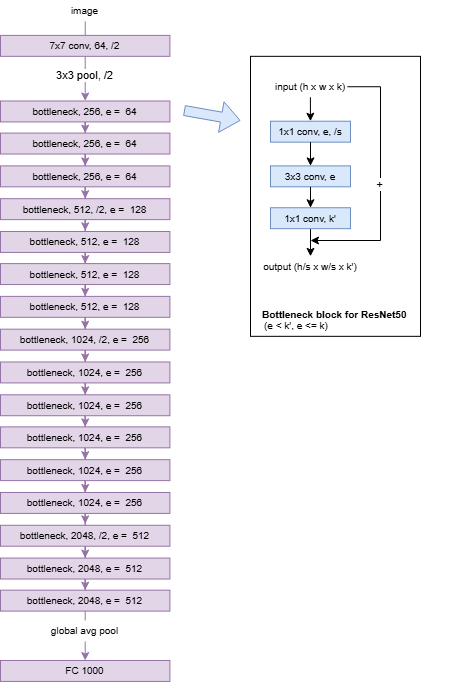
\includegraphics[width=0.5\linewidth]{images/LightCNN-D.drawio.png}
  \caption{Kiến trúc mạng ResNet50 }
  \label{fig:resnet50}
\end{figure}

Nhằm giải quyết bài toán hội tụ của các mô hình sâu trong giới hạn thời gian huấn luyện, ResNet \cite{ARC_He_2016_CVPR} được đề xuất dựa trên nhận định rằng việc xấp xỉ trực tiếp ánh xạ đồng nhất (identity mapping) bằng các lớp phi tuyến là không hiệu quả. Thay vì học trực tiếp hàm mục tiêu H(x), ResNet chuyển sang học hàm dư F(x)=H(x)−x, từ đó đầu ra được biểu diễn dưới dạng F(x)+x, hiện thực thông qua các shortcut connections dạng ánh xạ đồng nhất. Cách tiếp cận này không làm tăng đáng kể số lượng tham số hay chi phí tính toán (ngoại trừ phép cộng từng phần tử), qua đó cho phép các mạng sâu dựa trên ResNet duy trì độ phức tạp tính toán ở mức cho phép. Thực nghiệm cho thấy ResNet cho phép huấn luyện hiệu quả các mạng rất sâu, đồng thời đạt độ chính xác cao hơn khi độ sâu tăng lên. Kiến trúc mạng ResNet50 được minh họa ở Hình \ref{fig:resnet50}

\begin{table}[]
    \centering
    \small
    \begin{tabular}{|c|c|c|p{8cm}|}
        \hline
        \textbf{Kiến trúc} & \textbf{Năm} & \textbf{Độ sâu} & \textbf{Đóng góp chính} \\
        \hline
        SqueezeNet\cite{43_article} & 2016 & 18 & Fire module with squeeze and expand layer\\
        MobileNet\cite{ARC_howard_2017_mobilenets} & 2017 & 28 & Depthwise separable convolution \\
        ShuffleNetV1\cite{arc_Zhang_2018_CVPR} & 2018 & 50 & Pointwise group convolution and cơ chế channel shuffle\\
        ShuffleNetV2\cite{arc_Ma_2018_ECCV} & 2018 & 51 & Cơ chế channel split\\
        MobileNetV2\cite{ARC_Sandler_2018_CVPR} & 2018 & 53 & Cấu trúc Inverted residual bottleneck\\
        MobileFaceNet\cite{16_chen_2018_mobilefacenets} & 2018 & 50 & Global depthwise convolution \\
        MobiFace\cite{ARC_9185981} & 2019 & 46 & Chiến lược fast downsampling và fully connected layer thay cho GDC \\
        \hline
    \end{tabular}
    \caption{Tổng hợp các kiến trúc mạng CNN gọn nhẹ}
    \label{tab:Light-CNN}
\end{table}

Có thể nói sự phát triển của các mô hình nhận diện khuôn mặt nhìn chung bám sát tiến trình của các kiến trúc phân loại ảnh. Cụ thể, năm 2014, DeepFace sử dụng kiến trúc AlexNet và đạt được độ chính xác tiệm cận mức độ của con người, đánh dấu một cột mốc quan của lĩnh vực nhận diện khuôn mặt\cite{18_s25051410}. Tiếp theo đó, nhiều mô hình tiêu biểu được đề xuất như FaceNet (dựa trên GoogLeNet), VGGFace (dựa trên VGGNet), và SphereFace (dựa trên ResNet), góp phần nâng cao đáng kể độ chính xác của bài toán nhận diện khuôn mặt\cite{20_WANG2021215}.

Để đáp ứng yêu cầu triển khai trên thiết bị di động, hệ thống nhúng và các kịch bản thời gian thực, nhiều kiến trúc CNN gọn nhẹ đã được đề xuất (Bảng \ref{tab:Light-CNN}). Trong bài toán phân loại ảnh tổng quát, SqueezeNet \cite{43_article} là một trong những hướng tiếp cận tiên phong, đạt độ chính xác tương đương AlexNet trên tập ImageNet trong khi giảm số lượng tham số tới 50 lần, thông qua việc sử dụng fire module gồm lớp squeeze (tích chập 1×1) và lớp expand (kết hợp tích chập 1×1 và 3×3).
Bên cạnh đó, ShuffleNetV1 \cite{arc_Zhang_2018_CVPR} đề xuất sử dụng pointwise group convolution kết hợp với cơ chế channel shuffle nhằm giảm chi phí tính toán mà vẫn duy trì độ chính xác. ShuffleNetV2 \cite{arc_Ma_2018_ECCV} tiếp tục tối ưu hóa tốc độ suy luận bằng cách áp dụng phép channel split, cho phép duy trì số lượng kênh lớn với độ rộng cân bằng, đồng thời tránh các phép tích chập dày đặc và số lượng lớn nhóm trong group convolution. Song song đó, họ kiến trúc MobileNet \cite{ARC_howard_2017_mobilenets} và MobileNetV2 \cite{ARC_Sandler_2018_CVPR} đóng vai trò nền tảng cho nhiều mô hình nhẹ trong thị giác máy tính, nhờ việc sử dụng depthwise separable convolution để giảm đáng kể độ phức tạp tính toán. Dựa trên các kiến trúc này, các biến thể chuyên biệt cho bài toán xác minh khuôn mặt như MobileFaceNet \cite{16_chen_2018_mobilefacenets} và MobiFace đã được phát triển, và hiện được xem là những lựa chọn phổ biến cho các hệ thống nhận diện khuôn mặt trên thiết bị tài nguyên hạn chế.
\begin{figure*}[ht]
    \centering
    \begin{subfigure}[t]{0.15\textwidth}
        \centering
        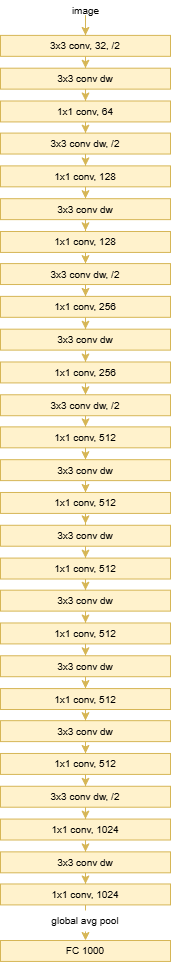
\includegraphics[width=\linewidth]{images/LightCNN.drawio.png}
        \caption{MobileNet}
        \label{fig:light_cnn_a}
    \end{subfigure}%
    ~
    \begin{subfigure}[t]{0.333\textwidth}
        \centering
        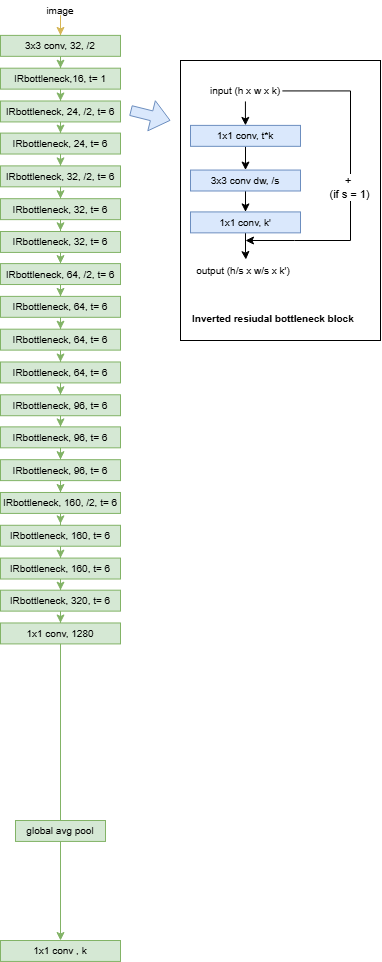
\includegraphics[width=\linewidth]{images/LightCNN-B.drawio.png}
        \caption{MobileNetV2}
        \label{fig:light_cnn_b}
    \end{subfigure}%
    ~
    \begin{subfigure}[t]{0.105\textwidth}
        \centering
        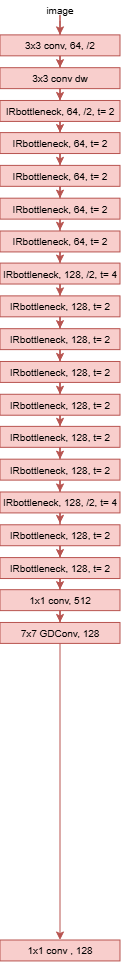
\includegraphics[width=\linewidth]{images/LightCNN-C.drawio.png}
        \caption{MobileFaceNet}
        \label{fig:light_cnn_c}
    \end{subfigure}%
        ~
    \begin{subfigure}[t]{0.105\textwidth}
        \centering
        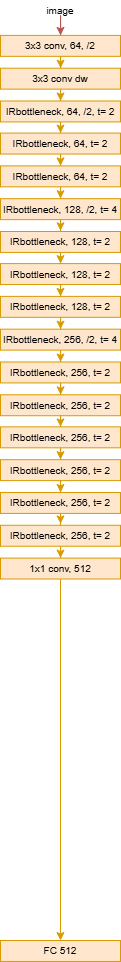
\includegraphics[width=\linewidth]{images/LightCNN-E.drawio.png}
        \caption{MobiFace}
        \label{fig:light_cnn_e}
    \end{subfigure}%
    
    \caption{Các kiến trúc mạng CNN gọn nhẹ dựa trên kiến trúc MobileNet}
\end{figure*}


Nhằm giảm độ phức tạp tính toán của tích chập truyền thống, MobileNet\cite{ARC_howard_2017_mobilenets} đề xuất sử dụng depthwise separable convolution làm khối xây dựng chính, kết hợp với hai siêu tham số để điều khiển kích thước mô hình. Cụ thể, phép tích chập được tách thành hai bước: depthwise convolution thực hiện lọc độc lập trên từng kênh đầu vào, và pointwise convolution (1×1) kết hợp các đặc trưng giữa các kênh. Cách phân tách này giúp giảm đáng kể chi phí tính toán, với độ phức tạp xấp xỉ $\frac{1}{N} + \frac{1}{D_K^2}$ so với tích chập chuẩn (trong đó $N$ là số kênh đầu ra và $D_K$ là kích thước kernel). Tương tự, số lượng tham số của một lớp giảm xuống còn $D_K \times D_K \times M + M \times N$, thấp hơn đáng kể so với tích chập truyền thống. Ngoài ra, MobileNet còn giới thiệu hai siêu tham số quan trọng là width multiplier và độ phân giải đầu vào, cho phép điều chỉnh linh hoạt giữa độ chính xác và chi phí tính toán. Kiến trúc tổng thể của mô hình được minh họa trong Hình \ref{fig:light_cnn_a}.

Dựa trên MobileNet, MobileNetV2\cite{ARC_Sandler_2018_CVPR} được đề xuất nhằm duy trì tính đơn giản đồng thời cải thiện độ chính xác và hiệu quả mô hình. Điểm cốt lõi của kiến trúc này là khối inverted residual bottleneck cho phép kết nối tắt giữa các lớp có số chiều thấp (bottleneck), tương tự cơ chế skip connection trong ResNet\cite{ARC_He_2016_CVPR}, qua đó giúp mô hình sâu hội tụ hiệu quả hơn. Cấu trúc này được thiết kế để hạn chế mất mát thông tin do các hàm phi tuyến gây ra trên không gian đặc trưng có số chiều thấp, được cho là chứa các thông tin quan trọng. Đồng thời, cấu trúc nghịch đảo còn giúp tối ưu bộ nhớ trong quá trình suy luận, phù hợp với các thiết bị có tài nguyên hạn chế. Thực nghiệm cho thấy MobileNetV2 đạt độ chính xác cao hơn so với MobileNet, đồng thời giảm số lượng tham số và số phép toán (MAdds), từ đó giảm độ phức tạp tính toán. Kiến trúc tổng thể của mô hình được minh họa trong Hình \ref{fig:light_cnn_b}.

Dựa trên nhận định rằng global average pooling trong MobileNet và MobileNetV2 làm suy giảm thông tin không gian (spatial information), dẫn đến hiệu năng chưa tối ưu trong bài toán xác minh khuôn mặt, MobileFaceNet \cite{16_chen_2018_mobilefacenets} đề xuất thay thế bằng lớp Global Depthwise Convolution (GDC). Đây là một phép depthwise convolution với kernel có kích thước bằng đầu vào, cho phép mỗi kênh đầu ra tổng hợp thông tin với trọng số khác nhau tương ứng cho từng đơn vị, từ đó bảo toàn đặc trưng không gian của khuôn mặt. Độ phức tạp và số lượng tham số của lớp này là $W \times H \times M$ (với $W, H$ là kích thước không gian và $M$ là số kênh), và do được áp dụng ở tầng tích chập cuối nên chi phí tính toán vẫn ở mức thấp. Thực nghiệm cho thấy mô hình đạt tốc độ suy luận nhanh và kích thước nhỏ cùng với độ chính xác 99.55\%, tiệm cận với các phương pháp tiên tiến nhất sử dụng kiến trúc quy mô lớn trên LFW (99.86\%)\cite{2_electronics9081188}.

Kiến trúc MobiFace \cite{ARC_9185981} được phát triển dựa trên MobileFaceNet, kết hợp chiến lược fast downsampling nhằm tăng tốc quá trình tính toán. Đồng thời, việc thay thế lớp Global Depthwise Convolution bằng lớp fully connected giúp cải thiện độ chính xác của mô hình, nhưng kéo theo sự gia tăng số lượng tham số và kích thước mô hình. Thực nghiệm cho thấy, mặc dù kích thước mô hình tăng lên khoảng 9.3 MB, thời gian suy luận của MobiFace vẫn nhanh hơn so với MobileFaceNet nhờ chiến lược fast downsampling. Ngoài ra, mô hình cũng đạt độ chính xác 99.72\% trên tập dữ liệu LFW.

Ngoài ra, để xây dựng các kiến trúc gọn nhẹ, có thể tối ưu các mô hình pretrained thông qua các kỹ thuật như knowledge distillation, network pruning, connectivity learning và low-rank factorization. Bên cạnh đó, tối ưu siêu tham số và Neural Architecture Search (NAS) cũng là các hướng tiếp cận được quan tâm. Đặc biệt, NAS cho phép tự động tìm kiếm kiến trúc mạng tối ưu dưới các ràng buộc về dữ liệu hoặc phần cứng, thay vì thiết kế thủ công\cite{14_10.1145/3776588}.
\subsubsection{Hàm kích hoạt}
\begin{table}[]
     \small
    \centering
    \begin{tabular}{|c|l|}
        \hline
        \textbf{Hàm kích hoạt} & \textbf{Định nghĩa}  \\
        \hline
        Sigmoid & $f(x) = (1+e^{-x})^{-1}$\\
        Tanh &    $f(x) = \frac{e^{x}-e^{-x}}{e^{x}-e^{-x}}$\\
        ReLU & $\displaystyle f(x) = \left\{ 
                  \begin{aligned}
                    x & \text{ if } x > 0 \\
                    0 & \text{ if } x \leq 0
                  \end{aligned} 
                    \right.$ \\ 
        LReLU\cite{LReLU_Maas2013RectifierNI} & $\displaystyle f(x) = \left\{ 
                  \begin{aligned}
                    x & \text{ if } x > 0 \\
                    0.01 * x & \text{ if } x \leq 0
                  \end{aligned} 
                    \right.$ \\ 
        PReLU\cite{PRELU_7410480} & $\displaystyle f(x) = \left\{ 
                  \begin{aligned}
                    x & \text{ if } x > 0 \\
                    a * x & \text{ if } x \leq 0
                  \end{aligned} 
                    \right. $ \\
        Maxout\cite{ACT_pmlr-v28-goodfellow13} & $f_{ij}(x) = \max\limits_{k\in [1,N]}(x^k_{ij})$\\
        MFM\cite{40_8353856} & $f_{ij}^k(x) = \max (x^k_{ij},x^{k+N}_{ij})$\\
        \hline
    \end{tabular}
    \caption{Tổng hợp các hàm kích hoạt phổ biến}
    \label{tab:activation_table}
\end{table}

Trong bài toán nhận dạng khuôn mặt, các hàm kích hoạt thường được sử dụng bao gồm sigmoid, tanh, ReLU và các biến thể của chúng (bảng \ref{tab:activation_table}). Trong đó, ReLU (Rectified Linear Unit) được xem là lựa chọn phổ biến nhất nhờ chi phí tính toán thấp, khả năng biểu diễn phi tuyến hiệu quả, đồng thời góp phần giảm hiện tượng vanishing gradient và thúc đẩy tính thưa (sparsity) của mạng.

Tuy nhiên, ReLU tồn tại hạn chế khi triệt tiêu toàn bộ các giá trị âm, có thể dẫn đến mất mát thông tin, đặc biệt ở các lớp tích chập đầu tiên. Ở các tầng này, đặc trưng học được thường tương đồng với các Gabor wavelets, trong đó cả thành phần âm và dương đều mang ý nghĩa quan trọng. Để khắc phục vấn đề này, nhiều biến thể của ReLU đã được đề xuất, tiêu biểu như Leaky ReLU (LReLU)\cite{LReLU_Maas2013RectifierNI} và Parametric ReLU (PReLU)\cite{PRELU_7410480}, cho phép duy trì một phần thông tin ở miền âm, qua đó cải thiện khả năng biểu diễn của mô hình.

\begin{figure}[ht]
  \centering
  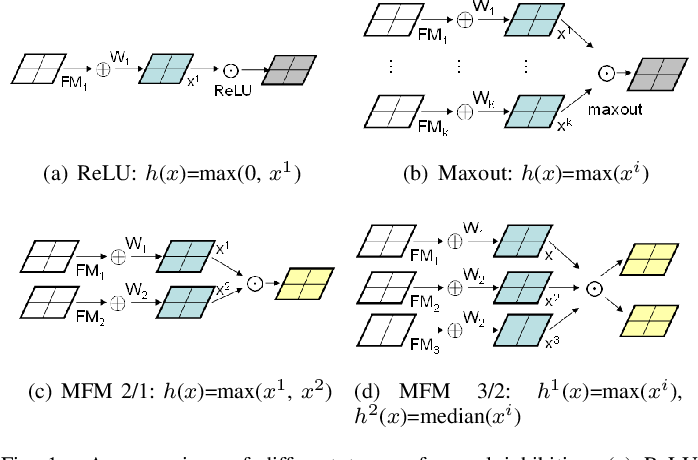
\includegraphics[width=\linewidth]{images/1-Figure1-1.png}
  \caption[Hàm kích hoạt MFM]{Hàm kích hoạt MFM trong tương quan với các hàm kích hoạt khác (Nguồn: \cite{40_8353856})}
  \label{fig:MFM}
\end{figure}

Nhằm xử lý vấn đề nhiễu nhãn (noisy label flips) trong các tập dữ liệu huấn luyện - yếu tố có thể làm suy giảm đáng kể hiệu năng mô hình - đồng thời duy trì tính gọn nhẹ của mô hình, Xi Wu et al.(2018)\cite{40_8353856} đã đề xuất hàm kích hoạt Max-Feature-Map (MFM), được phát triển dựa trên ý tưởng của Maxout. Tuy nhiên, khác với Maxout vốn hướng đến xấp xỉ một hàm lồi bất kỳ, MFM tập trung khai thác cơ chế cạnh tranh giữa các đặc trưng nhằm cải thiện khả năng tổng quát hóa (generalization). Cụ thể, MFM thực hiện phép toán cực đại trên các cặp hoặc nhóm nhỏ đặc trưng, thay vì trên toàn bộ không gian đặc trưng như Maxout. Với cơ chế này các mô hình sử dụng MFM không chỉ nhẹ hơn về mặt tính toán mà còn đạt được độ bền vững (robustness) cao hơn trong các điều kiện dữ liệu không lý tưởng. Cuối cùng, tác giả tích hợp MFM cùng với các bộ lọc kích thước nhỏ, kiến trúc Network in Network và các residual block để xây dựng các mô hình có kiến trúc gọn nhẹ. Các mô hình này được thực nghiệm trên nhiều bộ dữ liệu, trong đó đạt độ chính xác 99.33\% trên LFW và duy trì hiệu năng tốt trên các tập dữ liệu khác. Kết quả cho thấy rằng, dù có cấu trúc tối giản, các mô hình vẫn đạt khả năng tổng quát hóa cao, đặc biệt trong các kịch bản nhận diện khuôn mặt khác miền (cross-domain face recognition).
\subsection{Hàm mất mát}
Các hàm mất mát đóng vai trò then chốt trong việc quyết định độ chính xác của mô hình học sâu, thông qua việc định nghĩa hàm phạt giữa nhãn dự đoán và nhãn thực tế\cite{sota_GUO2019102805}. Ban đầu, các phương pháp truyền thống như softmax loss được sử dụng rộng rãi; tuy nhiên, trong bối cảnh số lượng lớp lớn và biến thiên nội lớp (intra-class variation) có thể vượt quá khác biệt liên lớp (inter-class variation), softmax không đủ khả năng tạo ra các đặc trưng có tính phân biệt cao\cite{20_WANG2021215}.

Do đó, việc thiết kế các hàm mất mát hiệu quả hơn nhằm cải thiện khả năng tổng quát hóa trở thành hướng nghiên cứu trọng tâm trong nhận diện khuôn mặt. Các nghiên cứu ban đầu tập trung vào các hàm mất mát dựa trên khoảng cách Euclid. Đến năm 2017, các phương pháp như NormFace nhấn mạnh tầm quan trọng của việc chuẩn hóa đặc trưng và trọng số, từ đó mở ra hướng tiếp cận dựa trên biên góc/cosine\cite{23_meng_2021_magface}. Cách tiếp cận này cho phép học các đặc trưng phân biệt trên không gian hình cầu (hypersphere manifold), phù hợp hơn với bản chất của dữ liệu khuôn mặt và mang lại cải thiện đáng kể về hiệu năng\cite{20_WANG2021215}. Gần đây, các phương pháp với adaptive margin được đề xuất, cho phép tự động điều chỉnh siêu tham số, tăng tính linh hoạt và nâng cao khả năng tổng quát hóa của hàm mất mát\cite{23_meng_2021_magface}. Các hàm mất mát phổ biến được tóm tắt trong Bảng \ref{tab:loss_table}.
\begin{table}[]
    \renewcommand{\arraystretch}{1.5}
    \small
    
    \centering
    
    \begin{tabular}{|p{2cm}|l|p{9cm}|}
        \hline
        \textbf{Phân loại} & \textbf{Hàm mất mát} & \textbf{Định nghĩa}  \\
        \hline
        Softmax& Softmax & $L = -\frac{1}{M}\sum_{i=1}^M log\frac{e^{W_{y_i}^Tx_i+b_{y_i}}}{\sum_{j=1}^N e^{W_j^T x_i+b_j}}$ \\
        \hline
        \multirow[c]{3}{2cm}{Dựa trên \newline khoảng cách Euclide}& Contrastive loss\cite{20_WANG2021215} & $L=\sum_{i,j=1}^M [\delta_{ij}\max(0,\lVert x_i-x_j\rVert_2-m^+) + (1-\delta_{ij})\max(0,m^- - \lVert x_i-x_j\rVert_2)]$\\
        & Triplet loss(2015)\cite{39_Schroff_2015_CVPR}& $L= \sum_{i=1}^M[\lVert x_i^a - x_i^p\rVert^2_2 - \lVert x_i^a - x_i^n\rVert^2_2 + m]$ \\
        & Center loss(2016)\cite{LOSS_Center_10.1007/978-3-319-46478-7_31} & $L = \frac{1}{2}\sum_{i=1}^M \lVert x_i-c_{y_i}\rVert^2_2$\\
        \hline
        \multirow[c]{4}{2cm}{Biến thể \newline của hàm softmax}
        & CoCo loss(2017) \cite{LOSS_liu2017rethinkingfeaturediscriminationpolymerization} & $L = -\sum_{i=1}^Mlog \frac{e^{\hat{c}_{y_i}^T\cdot \hat{x_i} }}{\sum_{j=1}^N e^{\hat{c}_{j}^T\cdot \hat{x_i}}}$\\
        & NormFace (2017)\cite{LOSS_Norm_10.1145/3123266.3123359} & $ L= -\frac{1}{M}\sum_{i=1}^Mlog(\frac{e^{s\hat{W}_{y_i}^T\hat{x}_i}}{\sum_{j=1}^N e^{s\hat{W}_{j}^T\hat{x}_i}})$ \\
        & L-softmax(2017)\cite{LOSS_L_liu_2017_largemargin}&  $L= -\frac{1}{M}\sum_{i=1}^Mlog(\frac{e^{\lVert W_{y_i}\rVert \lVert x_i \rVert \varphi(\theta_{y_i})}}{e^{\lVert W_{y_i}\rVert \lVert x_i \rVert \varphi(\theta_{y_i})}+\sum_{j\ne y_i}e^{\lVert W_{y_i}\rVert \lVert x_i \rVert cos(\theta_{j})}})$; $\varphi(\theta)=(-1)^kcos(m\theta)-2k, \theta\in [\frac{k\pi}{m}$, $\frac{(k+1)\pi}{m}]$\\
        & A-softmax(2017)\cite{10_Liu_2017_CVPR} & $L= -\frac{1}{M}\sum_{i=1}^Mlog(\frac{e^{\lVert x_i \rVert \varphi(\theta_{y_i})}}{e^{ \lVert x_i \rVert \varphi(\theta_{y_i})}+\sum_{j\ne y_i}e^{ \lVert x_i \rVert cos(\theta_{j})}})$; $\varphi(\theta)=(-1)^kcos(m\theta)-2k, \theta\in [\frac{k\pi}{m}$, $\frac{(k+1)\pi}{m}]$\\
        & Cosface(2018)\cite{6_Wang_2018_CVPR} & $L= -\frac{1}{M}\sum_{i=1}^Mlog(\frac{e^{s(cos(\theta_{y_i}) - m)}}{e^{ s(cos(\theta_{y_i}) -m)}+\sum_{j\ne y_i}e^{ s cos(\theta_{j})}})$\\
        & Arcface(2019)\cite{4_Deng_2019_CVPR} & $L= -\frac{1}{M}\sum_{i=1}^Mlog(\frac{e^{s(cos(\theta_{y_i}+m))}}{e^{ s(cos(\theta_{y_i}+m))}+\sum_{j\ne y_i}e^{ s cos(\theta_{j})}})$\\              
        \hline
        \multirow[c]{2}{2cm}{Adaptive margin}& MagFace(2021)\cite{23_meng_2021_magface} & $L= \frac{1}{M}\sum_{i=1}^M-log(\frac{e^{s(cos(\theta_{y_i}+mg(\lVert x_i \rVert)))}}{e^{ s(cos(\theta_{y_i}+mg(\lVert x_i \rVert)))}+\sum_{j\ne y_i}e^{ s cos(\theta_{j})}})+ \lambda_gg(\lVert x_i \rVert)$
        \\ &ElasticFace(2022)\cite{5_Boutros_2022_CVPR}  & $L= -\frac{1}{M}\sum_{i=1}^Mlog(\frac{e^{s(cos(\theta_{y_i}+E(m,\sigma)))}}{e^{ s(cos(\theta_{y_i}+E(m,\sigma)))}+\sum_{j\ne y_i}e^{ s cos(\theta_{j})}})$\\
        \hline
    \end{tabular}
    \caption[Tổng hợp các hàm mất mát phổ biến]{ Tổng hợp các hàm mất mát phổ biến. Trong đó, $x_i$ là vector đặc trưng của mẫu thứ $i$, $y_i$ là nhãn tương ứng, $m$ là hệ số margin, $c_j$ là vector trung tâm của lớp $j$, $M$ và $N$ lần lượt là số mẫu và số lớp trong tập huấn luyện, $W_j$ và $b_j$ là trọng số và bias của lớp $j$, và $s$ là hệ số tỉ lệ điều chỉnh bán kính trong không gian đặc trưng, $\hat{x}$ là vector x sau khi được chuẩn hóa theo chuẩn $L_2$. 
    }
    \label{tab:loss_table}
\end{table}

Ở giai đoạn đầu, nhằm thu hẹp khoảng cách nội lớp và gia tăng khoảng cách liên lớp trong không gian Euclid, các hàm mất mát dựa trên cặp hoặc bộ ba mẫu như contrastive loss và triplet loss\cite{39_Schroff_2015_CVPR} được đề xuất. Tuy nhiên, các phương pháp này phụ thuộc mạnh vào chiến lược chọn mẫu (sample mining) với việc lựa chọn không hiệu quả có thể gây mất ổn định trong huấn luyện. Đồng thời, với tập dữ liệu lớn, số lượng tổ hợp cặp/bộ ba tăng nhanh, dẫn đến chi phí tính toán cao. Để khắc phục, center loss\cite{LOSS_Center_10.1007/978-3-319-46478-7_31} được đề xuất dựa trên bài toán phân loại, với mục tiêu thu hẹp khoảng cách giữa đặc trưng và tâm (center) của lớp tương ứng. Tuy nhiên, phương pháp này vẫn tồn tại hạn chế như tiêu tốn bộ nhớ (đặc biệt ở lớp phân loại) và yêu cầu dữ liệu huấn luyện cân bằng, đủ mẫu cho mỗi danh tính.

Năm 2017, Wen et al. \cite{LOSS_Norm_10.1145/3123266.3123359} và các nghiên cứu liên quan đã chỉ ra tầm quan trọng của việc chuẩn hóa đặc trưng và trọng số trong bài toán nhận diện khuôn mặt. Cụ thể, khi học bằng softmax loss, độ lớn của vector đặc trưng thường phụ thuộc vào chất lượng ảnh đầu vào, trong khi thông tin định danh chủ yếu nằm ở hướng (hay góc) giữa các vector đặc trưng. Việc chuẩn hóa giúp loại bỏ ảnh hưởng của độ lớn, buộc mô hình học các đặc trưng phân biệt dựa trên khoảng cách góc trong không gian chuẩn hóa (đơn vị vòng tròn hoặc siêu cầu). Cách tiếp cận này phù hợp hơn với bản chất phân phối của dữ liệu khuôn mặt, đồng thời đặt nền tảng cho sự phát triển của các hàm mất mát dựa trên biên góc về sau. Tuy nhiên, cần lưu ý rằng Wang et al. (2018) \cite{loss_cmp_Wang_2018_ECCV} chỉ ra các hàm mất mát dựa trên biên góc/cosine nhạy cảm hơn với dữ liệu nhiễu, đặc biệt trong trường hợp nhãn bị sai (label flips), từ đó có thể làm suy giảm hiệu năng mô hình.

Trong số các hàm mất mát dựa trên biên góc/cosine, ArcFace được xem là một trong những phương pháp đạt hiệu năng cao nhất. Nghiên cứu của Hsu et al. (2020) \cite{25_Hsu_2020_CVPR_Workshops} cho thấy ArcFace vượt trội hơn CosFace và A-Softmax trong hầu hết các kịch bản như biến thiên tư thế, độ tuổi và che khuất, ngoại trừ trường hợp độ phân giải thấp. Ưu thế này đến từ đặc tính hình học rõ ràng của ArcFace, khi biên góc được thiết kế tương ứng trực tiếp với khoảng cách trắc địa trên siêu mặt cầu (hypersphere). Trong bài toán phân loại hai lớp, ArcFace tạo ra biên quyết định tuyến tính theo góc, trong khi A-Softmax và CosFace có biên phi tuyến, giúp ArcFace có khả năng hội tụ ổn định và hiệu quả hơn. Dựa trên ý tưởng tăng độ compactness nội lớp và khoảng cách góc liên lớp, ArcFace bổ sung một biên góc vào góc giữa vector đặc trưng và vector trọng số của lớp mục tiêu (mang ý nghĩa tương đồng với tâm của các lớp), bằng hàm mất mát:
\[ L = -\frac{1}{M}\sum_{i=1}^{M} \log \frac{e^{s\cos(\theta_{y_i}+m)}}{e^{s\cos(\theta_{y_i}+m)} + \sum_{j \ne y_i} e^{s\cos(\theta_j)}}\]

trong điều kiện các vector đặc trưng và trọng số đã được chuẩn hóa, và hệ số s được sử dụng để co giãn không gian đặc trưng, tránh phạm vi giá trị đầu vào của hàm Softmax quá hẹp. Nhờ đó, các embedding được phân bố trên mặt siêu cầu bán kính s. Với khả năng tối ưu trực tiếp khoảng cách trắc địa, độ chính xác cao và dễ triển khai, ArcFace đã trở thành một chuẩn mực trong các hệ thống nhận diện khuôn mặt hiện đại.
\begin{figure}[ht]
  \centering
  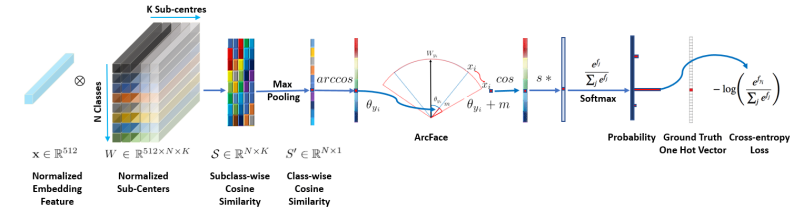
\includegraphics[width=\linewidth]{images/ArcFace.drawio.png}
  \caption[Hàm mất mát ArcFace]{Quá trình huấn luyện mô hình giám sát bởi hàm mất mát ArcFace (Nguồn: \cite{4_Deng_2019_CVPR})}
  \label{fig:arcface}
\end{figure}

Gần đây, dựa trên các hàm mất mát biên góc/cosine, nhiều phương pháp adaptive margin đã được đề xuất nhằm giảm phụ thuộc vào việc tinh chỉnh siêu tham số, đồng thời xử lý các vấn đề như dữ liệu mất cân bằng và overfitting, qua đó cải thiện khả năng tổng quát hóa. Tiêu biểu, ElasticFace \cite{5_Boutros_2022_CVPR} sử dụng phân phối Gaussian để lấy mẫu margin, giúp tăng tính linh hoạt và thích nghi với phân bố không đồng đều giữa các lớp. Trong khi đó, MagFace \cite{23_meng_2021_magface} khai thác độ lớn của vector đặc trưng - được xem như thước đo chất lượng mẫu - để điều chỉnh margin, từ đó giảm ảnh hưởng của các mẫu chất lượng thấp và hạn chế overfitting. Thực nghiệm cho thấy cả hai phương pháp đều cải thiện hiệu năng trong các kịch bản có biến thiên nội lớp lớn và bộ dữ liệu thách thức. Trên tập LFW, hai mô hình lần lượt đạt được độ chính xác là 99.82\% và 99.83\%.
\subsection{Tóm tắt kết quả}
Trong những năm gần đây, học sâu đã đạt được nhiều thành tựu đáng kể trong các bài toán học máy và nhận dạng mẫu, nhờ vào ba yếu tố chủ đạo: sự gia tăng năng lực tính toán của phần cứng, chi phí phần cứng giảm, và các tiến bộ quan trọng trong nghiên cứu thuật toán. Trong ba nhánh chính của học sâu, học có giám sát đóng vai trò trung tâm trong việc trích xuất đặc trưng phục vụ các nhiệm vụ xác minh danh tính. Đặc biệt, mạng nơ-ron tích chập đã chứng minh hiệu quả vượt trội trong nhận dạng ảnh và trở thành nền tảng cốt lõi của các hệ thống nhận diện khuôn mặt\cite{2_electronics9081188}.

Sự phát triển của các kiến trúc mạng xương sống, kết hợp với những cải tiến trong thiết kế hàm mất mát - từ Softmax, các phương pháp dựa trên khoảng cách như Triplet Loss, đến các hàm biên góc như ArcFace - đã nâng cao đáng kể khả năng phân biệt của các vectơ đặc trưng\cite{20_WANG2021215,23_meng_2021_magface}. Bên cạnh đó, các kỹ thuật như chuẩn hóa (regularization) và nén mô hình được nghiên cứu áp dụng nhằm giảm hiện tượng overfitting và tối ưu hóa khả năng triển khai trên các thiết bị tài nguyên hạn chế\cite{27_alzubaidi_2021_review}.

Mặc dù đạt độ chính xác cao trên các bộ dữ liệu chuẩn, các hệ thống học sâu vẫn đối mặt với nhiều thách thức trong môi trường không kiểm soát, như biến thiên cực đoan về tư thế, độ tuổi và hiện tượng che khuất\cite{18_s25051410,2_electronics9081188,sota_GUO2019102805}. Ngoài ra, yêu cầu về dữ liệu chất lượng cao và phân bố cân bằng là yếu tố quan trọng để đảm bảo hiệu suất ổn định và tính công bằng, tránh định kiến về nhân khẩu học. Mô hình học sâu cũng bộc lộ lỗ hổng trước các tấn công đối nghịch (adversarial attacks) và tấn công giả mạo, yêu cầu phát triển các phương pháp đối phó nhằm tăng tính an ninh của hệ thống\cite{18_s25051410,20_WANG2021215}. Cùng với đó, việc triển khai trên thiết bị di động và hệ thống nhúng với tài nguyên hạn chế (EdgeAI/TinyDL) yêu cầu sự phát triển các kiến trúc gọn nhẹ, cùng với kỹ thuật tìm kiếm kiến trúc tự động NAS và phương pháp nén hiệu quả\cite{14_10.1145/3776588,27_alzubaidi_2021_review,20_WANG2021215}.

\begin{sidewaystable}[]
    \footnotesize
    \centering
    \begin{tabular}{|c|c|c|c|c|c|p{4cm}|c|}
        \hline &\textbf{Mô hình} & \textbf{Năm} & \textbf{Tác giả} & \textbf{Kiến trúc} & \textbf{Hàm mất mát} & \textbf{Tập huấn luyện (images, identities)} & \textbf{Độ chính xác (\%)} \\
        \hline 
        1&DeepFace & 2014 & Taigman et al.\cite{deep_face_Taigman_2014_CVPR}& CNN-9& Softmax & Facebook (4.4 M,4 K) & 97.35 $\pm$ 0.25 \\ 
        2&FaceNet & 2015 & Schroff et al.\cite{39_Schroff_2015_CVPR} & GoogleNet & Triplet Loss & Google (200M, 8M)& 99.63 $\pm$ 0.09\\ 
        3&Center Loss& 2016 & Wen et al\cite{LOSS_Center_10.1007/978-3-319-46478-7_31}& LeNet & Center loss & CASIA WebFace\cite{yi_2014_learning} + CACD2000\cite{chen14cross} + Celebrity+\cite{liu_2015_deep} (0.7M, 17K) & 99.28\\ 
        4&L-Softmax & 2016 & Liu et al.\cite{LOSS_L_liu_2017_largemargin}& VGGNet-18 & L-Softmax& CASIA-WebFace (490K, 10K) &98.71\\ 
        5&NormFace & 2017 & Wang et al.\cite{LOSS_Norm_10.1145/3123266.3123359}& ResNet28 & Contrastive Loss & CASIA WebFace (494K, 10K) & 99.19 $\pm$ 0.008\\ 
        6&MobileFaceNet & 2018 & Chen et al. \cite{16_chen_2018_mobilefacenets} & MobileFaceNet &ArcFace & cleaned MS-Celeb-1M\cite{guo_2016_msceleb1m} (3.8M,85K)\cite{4_Deng_2019_CVPR} & 99.55\\ 
        7&Light CNN-29 &2018 &Wu et al.\cite{40_8353856}&Light CNN-29 & Softmax & cleaned MS-Celeb-1M(5M,79K) & 99.33\\ 
        8&SphereFace & 2018 &Liu et al.\cite{10_Liu_2017_CVPR}& ResNet64 & A-Softmax & CASIA WebFace (494K, 10K)& 99.42\\ 
        9&Cosface & 2018 & Wang et al.\cite{6_Wang_2018_CVPR} & ResNet64 & Large Margin Cosine Loss & CASIA WebFace (494K, 10K)& 99.7\\ 
        10&ArcFace & 2019 & Deng et al.\cite{4_Deng_2019_CVPR} &ResNet100 & ArcFace & MS1MV2(5.8M,85K) & \textbf{99.83}\\ 
        11 & MobiFace & 2019 & Duong et al.\cite{ARC_9185981} & MobiFace & L2-Norm + Cross entropy & cleaned MS-Celeb-1M (3.8M,85K) & 99.72\\
        12&MagFace &2021 &Meng et al. \cite{23_meng_2021_magface} & ResNet100 & MagFace & MS1MV2(5.8M,85K) & \textbf{99.83}\\ 
        13&ElasticFace &2022 &Boutros et al.\cite{5_Boutros_2022_CVPR}& ResNet100 & ElasticFace-Cos & MS1MV2(5.8M,85K) & 99.82\\ 
       \hline
    \end{tabular}
     \caption{Tổng hợp hiệu suất của một số mô hình phổ biến trên tập LFW }
    \label{tab:dcnn_table}
\end{sidewaystable}
\section{Các giải pháp học sâu nhận diện khuôn mặt trên thiết bị nhúng vi điều khiển}

Đồ án này tập trung khảo sát các mô hình học sâu triển khai trên thiết bị nhúng vi điều khiển với tài nguyên hạn chế, điển hình gồm vài trăm kB RAM và bộ nhớ flash, tần số hoạt động từ hàng chục đến hàng trăm MHz, và có thể không hỗ trợ đầy đủ phép tính như trên các máy tính đa dụng. Ngoài ra, các hệ thống vi điều khiển thường hạn chế sử dụng cấp phát bộ nhớ động (dynamic memory allocation) nhằm tránh hiện tượng phân mảnh heap, vốn đặc biệt nghiêm trọng trong điều kiện tài nguyên bộ nhớ hạn chế. Các mô hình mục tiêu thường được thiết kế với mức tiêu thụ năng lượng dưới 1 mW nhằm đảm bảo khả năng vận hành lâu dài bằng pin\cite{1_warden_2020_tinyml}. Trọng tâm của đồ án là phân tích và tổng hợp các nghiên cứu ứng dụng học sâu trong bài toán nhận diện khuôn mặt trên nền tảng này.

Qua khảo sát, có thể nhận thấy số lượng công trình nghiên cứu chuyên sâu về nhận diện khuôn mặt trên phần cứng siêu hạn chế vẫn còn tương đối khiêm tốn. Phần lớn các nghiên cứu hiện nay tập trung vào việc điều chỉnh và triển khai các mô hình sẵn có thay vì xây dựng mới hoàn toàn. Các hướng tiếp cận tiêu biểu bao gồm: (i) áp dụng transfer learning từ các kiến trúc mạng tích chập gọn nhẹ \cite{38_Zemlyanikin_2019_ICCV,35_10457480}; (ii) đề xuất các biến thể kiến trúc dựa trên các mô hình nền tảng \cite{37_s20216114,17_10128985}; và (iii) sử dụng các mô hình CNN đơn giản cho các bài toán quy mô nhỏ \cite{32_10.1145/3417308.3430273}. Một số nghiên cứu còn phát triển các nguyên mẫu hệ thống tích hợp khối thu thập năng lượng (energy harvesting), hướng tới các giải pháp hoạt động không cần pin. Bên cạnh thiết kế mô hình, các kỹ thuật tối ưu hóa như pruning, quantization và quản lý memory footprint hiệu quả đóng vai trò then chốt trong việc hiện thực hóa trên phần cứng hạn chế. Ngoài ra, các hướng tiếp cận tổng quát hơn trong lĩnh vực thị giác máy tính cho vi điều khiển, chẳng hạn như Neural Architecture Search (NAS) dành cho mô hình siêu nhẹ \cite{MCUNet_NEURIPS2020_86c51678}, cũng cho thấy tiềm năng áp dụng trong bài toán nhận diện khuôn mặt.

Zemlyanikin et al. (2019)\cite{38_Zemlyanikin_2019_ICCV} đề xuất một mô hình nhận diện khuôn mặt triển khai trên SoC sử dụng vi điều khiển RISC-V với 512 kB RAM. Mô hình lựa chọn kiến trúc SqueezeNet nhằm giảm số lượng tham số và tối ưu bộ nhớ, hạn chế nhu cầu lưu trữ các activation maps. Quá trình huấn luyện được thực hiện theo hướng transfer learning trên tập VGGFace2 dưới sự giám sát của hàm mất mát cross-entropy và lifted structured. Trong giai đoạn suy luận, khoảng cách L2 được sử dụng để so sánh các vector đặc trưng nhờ tính đơn giản và hiệu quả khi triển khai trên phần cứng hạn chế. Bên cạnh đó, tác giả đề xuất một phương pháp lượng tử hóa mới nhằm giảm thiểu suy hao độ chính xác, cùng với phương pháp tối ưu memory footprint của mô hình. Kết quả thực nghiệm cho thấy mô hình có kích thước khoảng 1.5 MB, đạt thời gian suy luận dưới 1 giây trên nền tảng GreenWaves Technologies GAP8 SoC, với độ chính xác đạt 93\% trên tập dữ liệu LFW.

Giordano et al. (2020)\cite{32_10.1145/3417308.3430273} đề xuất một hệ thống smart camera không sử dụng pin cho bài toán nhận diện khuôn mặt, có thể triển khai trên vi điều khiển Apollo3 của Ambiq (ARM Cortex-M) với dung lượng bộ nhớ 384 kB RAM và 1024 kB ROM. Mô hình CNN được thiết kế để nhận diện 5 đối tượng cố định. Đối với mô hình này tập huấn luyện trùng với tập vận hành, do đó dữ liệu huấn luyện đã được tăng cường (data augmentation) nhằm nâng cao đa dạng nội lớp, mô phỏng các biến thiên về góc chụp và điều kiện chiếu sáng, giúp tăng sự tổng quát hóa cho mô hình. Kiến trúc mạng được đề xuất gồm 7 lớp với 39.821 tham số, sử dụng hàm kích hoạt ReLU cho các lớp ẩn và softmax ở lớp đầu ra. Trước khi triển khai, mô hình được lượng tử hóa nhằm giảm chi phí tính toán và bộ nhớ. Kết quả thực nghiệm cho thấy mô hình có kích thước khoảng 111kB với thời gian suy lận 0.64s và đạt độ chính xác 93\% với ảnh đầu vào độ phân giải 30×40.

Li et al. (2020)\cite{37_s20216114} đề xuất một mô hình học sâu cho nhận diện khuôn mặt sử dụng ảnh trắng đen, triển khai trên bộ xử lý DSP lõi kép HT82V82 với 256 kB RAM. Mô hình FN13 được phát triển dựa trên kiến trúc FaceNet, gồm 15 lớp, trong đó các khối Inception-ResNet được tinh chỉnh để phù hợp với ràng buộc phần cứng, kết hợp với bước chuẩn hóa L2 tại đầu ra. Hàm mất mát được thiết kế theo hướng kết hợp center loss và softmax nhằm tăng tính compact nội lớp và gia tăng khoảng cách liên lớp trong không gian đặc trưng. Trong giai đoạn suy luận, tác giả đề xuất sử dụng khoảng cách Euclid cho bài toán one-shot recognition, trong khi khoảng cách Mahalanobis được áp dụng khi có nhiều mẫu trên mỗi lớp, theo công thức ($D^2 = (x-\mu)^TC(x-\mu)$, với x là vector đặc trưng, μ là vector trung bình của lớp, và C là ma trận hiệp phương sai. Kết quả thực nghiệm cho thấy mô hình đạt độ chính xác 98.41\% trên tập LFW khi sử dụng 3 mẫu cho mỗi lớp. Đồng thời, FN13 cho thấy ưu thế về độ phức tạp tính toán (FLOPs), mặc dù kích thước mô hình tăng so với FaceNet.

Li et al. (2023)\cite{17_10128985} đề xuất một mô hình học sâu nhẹ sử dụng kiến trúc MobileFaceNet có tích hợp cơ chế channel attention nhằm gán trọng số thích ứng cho các kênh đặc trưng, qua đó tăng cường khả năng trích xuất thông tin quan trọng, tránh ảnh hưởng bởi nhiễu. Mô hình cũng đề xuất sử dụng kiến trúc MobileFaceNet kết hợp với feature pyramid trong giai đoạn phát hiện khuôn mặt để xử lý hiệu quả biến thiên về tỷ lệ và khoảng cách. Hệ thống được triển khai trên nền tảng nhúng RV1126/RV1109 EVB được trang bị NPU, là nền tảng đánh giá nhằm kiểm chứng chức năng của chipset tương ứng. Đồng thời, các kỹ thuật nén mô hình như network pruning và quantization được áp dụng nhằm giảm chi phí tính toán trong khi vẫn duy trì độ chính xác. Kết quả thực nghiệm cho thấy phương pháp đề xuất cải thiện đáng kể thời gian suy luận và hạn chế suy giảm thông tin.

Chen et al. (2023)\cite{35_10457480} đề xuất một hệ thống kiểm soát truy cập đa phương thức (multimodal), kết hợp nhận diện cử chỉ và khuôn mặt trên nền tảng vi điều khiển. Đối với bài toán nhận diện khuôn mặt, tác giả áp dụng transfer learning từ mô hình tiền huấn luyện trên tập dữ liệu lớn, cụ thể là MobileNetV2 được cấu hình width multiplier = 0.05 nhằm giảm số lượng tham số và độ phức tạp tính toán. Trong quá trình fine-tuning, hầu hết các lớp trung gian được đóng băng, chỉ cập nhật các lớp đầu, cuối và output; đồng thời kỹ thuật dropout được sử dụng để hạn chế hiện tượng overfitting trên tập dữ liệu nhỏ. Kết quả thực nghiệm cho thấy hệ thống có thể nhận diện chính xác các mẫu đã biết trên thiết bị biên với độ tin cậy trên 90\% trong khoảng 1 giây, trong khi các mẫu chưa biết chỉ đạt khoảng 70\%, cho phép thiết lập ngưỡng để xử lý bài toán nhận diện open-set. Tuy nhiên, hệ thống vẫn tồn tại hạn chế trước các hình thức tấn công giả mạo như là sử dụng ảnh. Mô hình đạt thời gian suy luận khoảng 640 ms với mức tiêu thụ năng lượng xấp xỉ 287 mJ cho ảnh đầu vào là trắng đen và có kích thước 96×96. Ngoài ra, tác giả đề xuất một workflow triển khai thực tế, trong đó dữ liệu khuôn mặt được thu thập qua ứng dụng, gửi lên máy chủ để huấn luyện, sau đó nén mô hình và cập nhật xuống thiết bị biên thông qua cơ chế over-the-air (OTA).

Tóm lại, lĩnh vực nhận diện khuôn mặt trên vi điều khiển đang phát triển mạnh theo hướng Tiny Deep Learning với các kiến trúc CNN siêu nhẹ, nhằm tối ưu hóa cân bằng giữa độ chính xác và giới hạn tài nguyên phần cứng. Các mô hình tiêu biểu (Bảng \ref{tab:tinycnn_table}) chủ yếu là các biến thể của MobileNet, MobileFaceNet, SqueezeNet và các mạng CNN tối giản. Để triển khai hiệu quả trên các nền tảng như ARM Cortex-M, ESP32 hay RISC-V, các kỹ thuật nén mô hình - bao gồm quantization, pruning và knowledge distillation - giữ vai trò then chốt trong việc giảm chi phí tính toán và dung lượng bộ nhớ trong khi vẫn duy trì hiệu năng. Kết quả thực nghiệm cho thấy các hệ thống này có thể đạt độ chính xác trên 92\% với thời gian suy luận từ vài mili giây đến dưới 1 giây, đáp ứng yêu cầu vận hành trong các ứng dụng thực tế như kiểm soát truy cập và giám sát tại biên.

\begin{sidewaystable}[]

    \centering
    \begin{tabular}{|c|c|c|p{3cm}|p{3cm}|p{3.5cm}|c|p{3cm}|}
        \hline &\textbf{Tác giả} & \textbf{Năm} & \textbf{Kiến trúc} & \textbf{Hàm mất mát} & \textbf{Tập huấn luyện (images,identities)} & \textbf{Độ chính xác (\%)} & \textbf{Phần cứng triển khai} \\
        \hline 
        
        1& Zemlyanikin et al. \cite{38_Zemlyanikin_2019_ICCV}& 2019 & SqueezeNet 1.1 & Cross Entropy + Lifted Structured Loss & VGGFace2(3.31M, 9.1K)\cite{cao_2018_vggface2} & 93.0 (LFW) & GreenWaves GAP8 (RISC-V)\cite{greenwavestechnologies_2019_gap8}  \\ 
         2 & Giordano et al. \cite{32_10.1145/3417308.3430273}& 2020 & CNN-7 & Categorical cross-entropy & CelebA (202.6K,10.2K)\cite{liu2015faceattributes} & 93.0 (CelebA)& ARM Cortex-M4F\cite{ambiqmicroinc_2024_apollo3} \\
         3& Hsiao-Chi Li et al. \cite{37_s20216114} & 2020 & Modified FaceNet & Center Loss + Softmax Loss &  CASIA WebFace (494K, 10K)  & 98.41 (LFW)& HT82V82 (Holtek)\cite{holtek_2017_holtek}\\ 
        4 & Wei Li et al. \cite{17_10128985} & 2023  & MobileFaceNet + Channel Attention & - & WIDER FACE(32,2K,-)\cite{yang2016wider} & 92.4 (Wider Face)& RV1126/RV1109 EVB\cite{fuzhourockchipelectronicscoltd_2020_rockchip} \\
        5 & Zijie Chen et al. \cite{35_10457480} & 2023 & MobileNetV2  & - & 2500 ảnh private & -  & ESP32-S \\ 

       \hline
    \end{tabular}
     \caption{Tổng hợp hiệu suất của một số mô hình học sâu trên thiết bị vi điều khiển }
    \label{tab:tinycnn_table}
\end{sidewaystable}